\chapter{Advances and Limitations in Open Source Arabic-Script OCR: A Case Study}
\chaptermark{Advances in Arabic OCR: A Case Study}
\label{ch:champs}
\thispagestyle{empty}
\vfill
This chapter has been accepted for publication as \fullcite{kiessling2020champs}.
\newpage

\section*{Abstract}
This work presents an accuracy study of the open source OCR engine, Kraken, on
the leading Arabic scholarly journal, al-Abhath. In contrast with other
commercially available OCR engines, Kraken is shown to be capable of producing
highly accurate Arabic-script OCR. The study also assesses the relative
accuracy of typeface-specific and generalized models on the al-Abhath data and
provides a microanalysis of the “error instances” and the contextual features
that may have contributed to OCR misrecognition. Building on this analysis, the
paper argues that Arabic-script OCR can be significantly improved through (1) a
more systematic approach to training data production, and (2) the development
of key technological components, especially multi-language models and improved
line segmentation and layout analysis.  

\section{Introduction}

In late 2017 JSTOR initiated a collaboration with the Open Islamicate Texts
Initiative (OpenITI) to run an Optical Character Recognition (OCR) pilot for
the JSTOR Arabic digitization feasibility study (funded through a generous
grant by the National Endowment for the Humanities).\footnote{OpenITI is a
multi-institutional initiative that is focused on building digital
infrastructure for the computational study of the texts of the Islamicate
world. It is currently led by Dr. Matthew Thomas Miller (Roshan Institute for
Persian Studies, University of Maryland, College Park), Dr. Sarah Bowen Savant
(Aga Khan University, London), and Dr. Maxim Romanov (University of Vienna).
Benjamin Kiessling (University of Leipzig/Université PSL) is one of OpenITI’s
primary computer science collaborators and he served as the technical lead for
the OpenITI JSTOR OCR pilot.  More information on the OpenITI project are
available on the project’s website: \url{https://openiti.org/about}. More
information on JSTOR’s NEH-funded project can be found here:
\url{https://about.jstor.org/news/jstor-receives-50000-neh-grant/}.}
 The problem that JSTOR had encountered in their feasibility study was the
problem that has long plagued efforts of scholars and librarians to digitize
Arabic, Persian, Urdu, and Ottoman Turkish print documents: Arabic-script OCR
programs produce notoriously poor results, despite the optimistic claims of
some of their marketing materials\cite{alghamdi2017experimental}.\footnote{Mansoor
Alghamdi and William Teahan open their 2017 study by noting that “although
handwritten script is significantly more challenging than printed Arabic text
for OCR, Arabic printed text OCR still poses significant challenges.” After
evaluating Sakhr, Finereader, RDI Clever Page, and Tesseract (3)—the main
options for Arabic-script OCR—on Arabic print works they conclude that “all the
evaluated Arabic OCR systems have low performance accuracy rates, below 75 per
cent, which means that the time which would take to manually correct the OCR
output would be prohibitive.” These results are consonant with the PIs’ own
experience using these OCR engines and those of our colleagues in the field of
Islamicate Studies.}
In addition to these programs’ lackluster performance, they also are not ideal
systems for academic users for other reasons as well - for example, several are
prohibitively expensive (for the average academic) and they offer little out of
the box trainability (i.e., they come only with a generic OCR model and they
cannot be trained to recognize new typefaces).

With these problems in mind, in 2016 OpenITI began working on the development
of open source OCR tools for Arabic-script languages (in print form) in
collaboration with the computer scientist Benjamin Kiessling.\footnote{To date
our work has primarily focused on Arabic-script OCR for print documents since
handwritten text recognition (HTR) for Arabic-script manuscripts presents a
series of additional issues (e.g., even more complex line segmentation and page
layout analysis problems, a dizzying array of different script styles and
scribal hands). However, we have begun preliminary experiments on Persian and
Arabic manuscripts with some promising initial results using distantly
supervised methods of training data production and the new line segmentation
methods developed by Kiessling \cite{kiessling2019badam}. See also the
experiments on HTR for Arabic manuscripts led by the British Library
\cite{clausner2018icfhr,rasm2019res,rasm2020trans}).}

 OpenITI’s first OCR study with the new open source OCR engine, Kraken,
developed by Kiessling, demonstrated that it was capable of achieving Arabic
script-only accuracy rates >97.5\% with as little as 800-1,000 lines of
training data for that document’s typeface
\cite{kiessling2017important}.\footnote{Training data, in the context of OCR,
consists of pairs of scans of individual lines of text with their digital
transcription.} OpenITI has also replicated these high accuracy rates on
Persian texts, with Perso-Arabic script-only accuracy rates ranging from 96.3\%
to 98.62\% with typeface-specific models.\footnote{This work has not been
published yet, but the full CER reports for these tests can be viewed at
OpenITI’s GitHub repository:
\url{https://github.com/OpenITI/OCR_GS_Data/tree/master/fas}.}

In this work, we present the results of our OCR study done in collaboration
with JSTOR on the al-Abhath Arabic journal (arguably the most important Arabic
language scholarly journal in the Middle East). In contrast with many OCR
accuracy reports, in this study we performed both detailed manual and automatic
Character Error Rate (CER) accuracy checks, which enabled us to develop a much
more fine-grained understanding of where the Kraken OCR engine was failing to
properly transcribe the Arabic text. These results confirm Kraken’s ability to
produce highly accurate Arabic-script OCR, but they also provide new insights
into the importance of systematic training data production, the relative
accuracy of typeface-specific and generalized models, and the key technological
improvements needed for improved Arabic-script OCR output. 

Section two reviews the open-source software used in this study before the
JSTOR Arabic OCR pilot and accuracy study are described in sections three and
four, respectively. Section five contains our recommendations for the necessary
technological and data improvements needed to improve Arabic OCR in the future.  
 
\section{OpenITI OCR Software: Kraken}

Kraken is an open-source OCR engine that was developed by Benjamin Kiessling.
It utilizes a segmentationless sequence-to-sequence approach
\cite{graves2006connectionist} with a hybrid convolutional and recurrent neural
network to perform character recognition \cite{kiessling2019kraken} which
obviates the need for character-level segmentation—i.e. the neural network
responsible for text extraction from image data recognizes whole lines of text
without resorting to smaller subunits like words or characters which can be
difficult to accurately compute for languages written in connected script. 

As an initial preprocessing step page images are converted into black and white
through a process called binarization. Layout analysis, i.e. the detection of
lines for subsequent steps, is then performed on this binarized image with an
algorithm based on traditional computer vision methods. In a final step, the
previously detected rectangular lines are fed into the neural network for
character recognition.\footnote{More on Kraken’s technical details can be
found here: \url{https://github.com/mittagessen/kraken}.}

The benefit of eliminating fine-grained segmentation in comparison to older
character segmenting systems such as tesseract 3, Sakhr, and most likely Abbyy
FineReader\footnote{As a proprietary software the exact nature of the
classifier is unknown.} is not only expressed during recognition but also
through easier to produce training data for adaptation of the OCR system to new
scripts and typefaces. With character-based systems annotators have to manually
locate and transcribe single characters while Kraken is trained on full line
transcriptions which are faster to annotate and verify, especially in the case
of connected scripts.

\section{The OpenITI JSTOR OCR Pilot}

OpenITI began the JSTOR OCR pilot by performing a randomized review of the
Arabic typefaces used in each year of the al-Abhath journal. The page images of
the journal were obtained from the Arabic and Middle Eastern Electronic Library
(Project AMEEL) of Yale University Library.\footnote{Project AMEEL’s website is
available here:
\url{http://www.library.yale.edu/ameeljournals/ameel_steps.html}.} It was
determined that there were two basic typefaces in the al-Abhath journal
archive, with the first typeface being much more prevalent than the second.
Examples of these two typefaces can be seen in figures 1-2 (for comparison
sake, the last word in both lines - on the left of the page - is the same
word).

\begin{description}
	\item[Typeface \#1] volumes 1-33, 36-39, 48-50
	\item[Typeface \#2] volumes 34-35, 40-47
\end{description}

\begin{figure}[h]
	\centering
	\begin{subfigure}{\textwidth}
	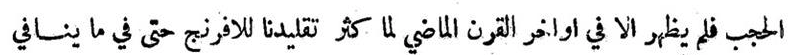
\includegraphics[width=\linewidth]{images/image8.png}
	\caption{Typeface \#1 sample}
	\label{fig3:fig1}
	\end{subfigure}
	\vskip\baselineskip
	\begin{subfigure}{\textwidth}
	
\includegraphics[width=\linewidth]{images/image9.png}
	\caption{Typeface \#2 sample}
	\label{fig3:fig2} 
	\end{subfigure}
	\caption{Sample of the two typefaces}
\end{figure}

Both typefaces had some internal font differences and other minor
character/script variations (e.g., patterns of use of alef hamza, slight shifts
in placement of dots, slight differences in the degree of curvature of lines in
a couple of instances, and minor ligature differences). This intra-typeface
variation was especially apparent in typeface \#1, which had a long run as
al-Abhath’s typeface. To address this issue it was decided that the best
approach would be to produce approximately 5,000 lines of training data for the
first typeface and 2,000 lines of training data for the second typeface. 

After a randomized sample of the pages representing each typeface were
selected, research assistants working with the OpenITI team produced the
training data for these 7,000 lines using CorpusBuilder 1.0 (a new OCR
postcorrection platform produced through the collaboration of OpenITI and
Harvard Law School’s SHARIAsource project).\footnote{For more on CorpusBuilder
1.0, please see: \url{https://www.openiti.org/projects/corpusbuilder}.} After
these 7,000 lines of training data were double checked for accuracy, a final
spot review was conducted. This “gold standard” data was then utilized for
model production and OCR.\footnote{This training data is available for reuse
and can be found in the OCR Gold Standard Training Data repository on OpenITI’s
Github page: \url{https://github.com/OpenITI/OCR_GS_Data}.}

The first round of OCR accuracy tests were performed by an outside contractor,
which JSTOR hired to conduct a ten-page manual accuracy comparison between the
Kraken output and the corresponding output for ABBYY (see Table~\ref{tab_champs:table_1}).

\begin{table}[h!]
\begin{center}
\caption{Contractor's accuracy comparison of Abbyy and OpenITI (Kraken) OCR results}
\label{tab_champs:table_1}
	\begin{tabularx}{\textwidth}{p{2.7cm}XXXXX} \toprule
& \textbf{Total number of characters} & \textbf{Abbyy character errors} & \textbf{OpenITI character errors} & \textbf{Abbyy character accuracy} & \textbf{OpenITI character accuracy}\\\midrule
Page \#1 \scriptsize{(00010004\_187997831.tif)} & 1230 & 270 & 38 & 78.049\% & \textbf{96.911\%} \\
Page \#2 \scriptsize{(00010004\_187997832.tif)} & 37& 15 & 27 & \textbf{59.459\%} & 27.027\%\\
Page \#3 \scriptsize{(00010031\_187998459.tif)} & 3182 & 355 & 23 & 88.843\% & \textbf{99.277\%}\\
Page \#4 \scriptsize{(00010063\_187999338.tif)} & 3157 & 327 & 29 & 89.642\% & \textbf{99.081\%}\\
Page \#5 \scriptsize{(00010129\_188001031.tif)} & 3222 & 378 & 16 & 88.268\% & \textbf{99.503\%}\\
Page \#6 \scriptsize{(00010012.tif)} & 3259 & 326 & 75 & 89.997\% & \textbf{97.699\%}\\
Page \#7 \scriptsize{(00010030.tif)} & 2503 & 230 & 17 & 90.811\% & \textbf{99.321\%}\\
Page \#8 \scriptsize{(00010126.tif)} & 2631 & 252 & 170 & 90.422\% & \textbf{93.539\%}\\
Page \#9 \scriptsize{(00010127.tif)} & 2294 & 223 & 35 & 90.279\% & \textbf{98.474\%}\\
Page \#10 \scriptsize{(00010132.tif)} & 2296 & 243 & 96 & 89.416\% & \textbf{95.819\%}\\
\bottomrule
\end{tabularx}
\end{center}
\end{table}

With the exception of page \#2, OpenITI (Kraken) performed substantially better
on the pages the contractor reviewed, achieving >99\% accuracy in 4/10 pages,
>97\% accuracy in 6/10 pages, >95.8\% in 8/10 pages. The exception to these
generally impressive numbers were pages \#2 and \#8 in which OpenITI (Kraken)
only achieved 27.027\% and 93.539\% respectively. While the contractor’s review
was quite useful and generally confirmed OpenITI’s results from its previous
work (i.e., that Kraken achieves significantly higher accuracy rates on Arabic
texts than the commercial OCR solutions for Arabic), the OpenITI team
discovered upon further review that there were several problems with the
contractor’s study.\footnote{For OpenITI previous study on Kraken, please see:
\cite{kiessling2017important}.}

\begin{wrapfigure}{O}{0.33\textwidth}
	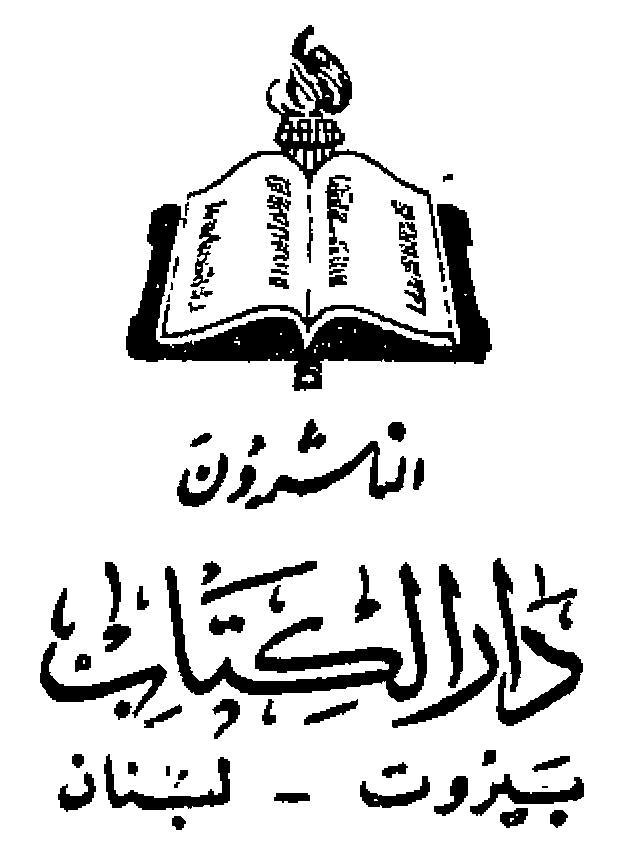
\includegraphics[width=0.3\textwidth]{images/image18.jpg}
	\caption{Header}
	\label{fig3:fig3}
\end{wrapfigure}

First, Page \#2 - by far the most disappointing result - is a highly atypical
page of al-Abhath data. It only contains 37 characters total and much of these
are contained in a large header that is in a highly calligraphic script and is
heavily vocalized (with diacritics) (see figure~\ref{fig3:fig3}). It is
noteworthy that Abbyy performed better on this script, but this page is an
extreme outlier in the data.

The second issue that we identified in the contractor’s review was that they
were marking certain differences between the original scans and OCR output as
errors which were not true errors, and, in some cases, even marked some
characters in the OCR output as errors that were not errors at all. For
example, in the former case, they marked all numbers as errors in the OpenITI
OCR output which were rendered as western Arabic numerals (e.g., 1, 2, 3)
instead of as eastern Arabic numerals (e.g.,\textarabic{١,٢,٣}) - a problem
that was particularly prevalent on page \#8 (thus at least partially
responsible for OpenITI’s comparatively lower accuracy rate on page \#8). The
OCR rendered them as western Arabic numerals instead of eastern Arabic numerals
because we decided to merge western and eastern Arabic numerals into their
universal numerical values in the OCR process and then represent that value in
western Arabic numerals in the OCR output.\footnote{This practice of collapsing
numeric values to their universal numerical value can be done for multiple
reasons, but, in this particular case, one of our primary motivating factors
was the fact that there were inconsistencies in the transcription practice of
numbers in the training data.} These differences, thus, are not true
errors—their numerical value is correct—and their representation can be changed
to eastern Arabic numerals if that is what users prefer. Another similar issue
was discovered in the contractor’s treatment of diacritics: they routinely
marked correctly rendered words as incorrect if the word’s original diacritics
were not included in the OCR output. However, again, this difference in the
original text and the OCR output is not a true error in transcription because
OpenITI has followed the practice (with one exception discussed further below)
of not reproducing diacritics in its training data (for reasons elaborate
below) and thus the fact that the diacritics were not rendered in OpenITI’s OCR
output is actually a sign that the Kraken OCR engine was functioning correctly.
(This training data generation practice can be changed if the users desire, and
given the results in OpenITI’s larger accuracy study described below, this
change may be advisable in the future, depending on the requirements of each
individual user’s use case.)

These problems in the contractor’s approach to error designation led them to
calculate lower accuracy estimates for OpenITI OCR output than it achieved in
actuality - a problem that was particularly accentuated in the case of page \#8,
which contained a larger amount of numbers than the other pages the contractor
reviewed. Due to the problems discovered in the contractor’s initial accuracy
study, JSTOR requested that OpenITI perform a more detailed accuracy assessment
on approximately fifty pages. 

\section{OpenITI Accuracy Study}

The OpenITI team began by generating automatic character error rate (CER)
reports for the al-Abhath data (see Table~\ref{tab_champs:table_2} for full
results).\footnote{The full CER reports can be found in the following OpenITI
Github repository:
\url{https://github.com/OpenITI/OCR_GS_Data/tree/master/ara/abhath}.} In the
first round of experiments, we built two different models—typeface model \#1
and \#2—based on the two different sets of training data produced for the two
typefaces that we identified in the full run of al-Abhath. After extracting
1,000 lines of training data from the original 5,000 lines for typeface \#1 and
700 lines of training data from the original 2,000 lines for typeface \#2 to
use as validation sets, we then trained the model on the remaining lines and
tested these models’ accuracy using the validation sets.\footnote{This method
of isolating a fixed number of lines of the training data as a validation set
for automatic accuracy testing is a standard procedure when evaluating machine
learning models.} These accuracy results can be found in rows 2-3 in
Table~\ref{tab_champs:table_2}.  These typeface-specific models were the ones
used to produce the OCR output that was transferred to JSTOR and that the
contractor reviewed for their accuracy study.

In the time between the delivery of the al-Abhath OCR output to JSTOR and
OpenITI’s manual accuracy study (discussed below), we began developing a
generalized Arabic model from all of the training data that OpenITI has
produced over the last year two years (circa 15,000 lines).\footnote{All of
this gold standard training data can be found here:
\url{https://github.com/OpenITI/OCR_GS_Data}.} (Generalized OCR models
incorporate character features from all of the typefaces represented in the
data upon which it is trained and therefore can often achieve higher levels of
accuracy on a broader range of typefaces.) We decided to test this model on all
of the al-Abhath data to determine if total OCR accuracy could be improved and,
if so, by how much. The results, shown in row \#4 of Table~\ref{tab_champs:table_2}, were
impressive.\footnote{For this accuracy assessment, 2,096 lines of the 7,000
lines of training data were isolated as a validation set.} The generalized
model’s  total character accuracy rate was 97.41\% - a 2.57 percentage point
improvement over the typeface \#2-only model (i.e., a ~50\% improvement rate)
and 1.45 percentage point improvement over the typeface \#1-only model - and
its Arabic script-only accuracy went up to a respectable 98.46\%. The
generalized model performed better than the typeface-specific models in all
categories, but its most significant gains were in the category of “inherited”
characters.

\begin{table}[h!]
\centering
\begin{minipage}{\textwidth}
\caption{Overview of OCR accuracy rates (drawn from character error rate (CER) reports}
\label{tab_champs:table_2}
\renewcommand\footnoterule{}
\begin{tabularx}{\textwidth}{lp{2cm}p{2cm}p{2cm}p{2cm}} \toprule
	& \textbf{Total\newline character accuracy} & \textbf{Arabic script only accuracy} & \textbf{Common character accuracy}\footnote{"Common characters” are characters shared by multiple scripts, primarily punctuation and other signs and symbols. In Arabic script,
	the kashīda or tatwīl (elongation character) is included in common script class.} & \textbf{Inherited character accuracy}\footnote{“Inherited characters” are characters, such as diacritics, that can be used on multiple languages and they only come to be defined in reference to the character with which they are combined (i.e., they “inherit” the script of the base character with which it is used).}\\\midrule
Typeface \#1 Model & 95.96\% & 97.56\% & 96.91\% & 79.67\%\\ 
Typeface \#2 Model & 94.84\% & 97.11\% & 94.16\% & 85.18\% \\
Generalized Model & 97.41\% & 98.46\% & 96.36\% & 89.44\%\\
\bottomrule
\end{tabularx}
\end{minipage}
\end{table}

\label{s:whitespace}
According to the CER reports, the most significant source of errors in both the
typeface \#2 model and the generalized model were whitespace (spacing) errors
and the Arabic diacritic, fatḥa tanwīn (unicode codepoint: Arabic fatḥatan). In
the case of the typeface \#1 model, whitespace errors were again the most
significant source of errors, followed by kāf (\textarabic{ك}), yā’ (\textarabic{ي}), and then fatḥa
tanwīn errors. The hamza above (\textarabic{ء}) character ranks as the seventh most common
error in typeface \#1 model and fifth in typeface \#2 model. The mīm (\textarabic{م})
character also is a common error in both the typeface \#1 and \#2 models, ranking
as the sixth and fifth most common error in their CER reports
respectively.\footnote{ Again, the full CER reports can be found in the
following OpenITI Github repository:
\url{https://github.com/OpenITI/OCR_GS_Data/tree/master/ara/abhath}.}

Concurrent with the generation of CER reports, the OpenITI team began a far
more expansive manual review of fifty—randomly selected—pages of the original
OCR output produced by the typeface \#1 and typeface \#2-specific models. Each of
these fifty pages were reviewed and then their error reports were collated into
a master list of 1,096 total error instances.\footnote{We use the term “error
instance” here to highlight the fact that we are not exclusively recording
individual, one-to-one character errors, but instances in the text in which one
or more characters were read incorrectly. In most cases, this is a one-to-one
character mistranscription, but in some other cases one character in the
original was read as two or more in the OCR output or multiple characters in
the original were read as one or none in the OCR output. In a few cases -
discussed in more detail below -there are whole sections of text that are
severely mistranscribed due to one or another feature in the original text.}
Finally, each error instance was examined with an eye towards identifying
possible factors in its adjacent context that may have led to that error and
coded the error instances with any of the following categories that were
applicable:

\begin{enumerate}
	\item Poor scan quality: an element in the raw scan is unclear, or extraneous marks are present.
	\item Ligature/atypical letter or dot form: connection between letters or placement of dots is in a less common form.
	\item Diacritics: diacritics were present in original word.
	\item Kashīda/tatwīl (elongation character): error appears in the context of a word that has been elongated. 
	\item Header/font alteration: bolded, italicized, or enlarged text.
	\item Footnote: error appears in the context of a footnote.
	\item Format: atypical format of presentation, e.g., table, list.
	\item Hamza: mistranscribed character was a hamza or a hamza was present in the original word that was mistranscribed.
	\item Doubled character: a single letter or number in the original scan was doubled in the OCR output.
	\item Missed fatḥa tanwīn: fatḥa tanwīn in the original text was not transcribed.
	\item Punctuation or other symbol: error was a punctuation mark or other symbol.
	\item Non-Arabic language: original text was not Arabic.
	\item Numbers: error was a number.
	\item Superscript numerals: error was a footnote numeral in the body of the text.
\end{enumerate}

This list of error codes is a mixture of error types (\#8-14) and the most
common recurring contextual features of the errors (\#1-7). For categories of
the latter type, it is important to emphasize that the presence of any of these
contextual features near an error in the original text does not necessarily
mean that it caused the error. But their repeated co-occurrence may be related
and thus suggest future avenues of research and/or the need to better address
this issue in the process of future training data production. We should also
point out that in the case of some errors none of the following category codes
were applicable, which only means that the reason for their improper rendering
was not immediately evident to the human reviewers. 

We do want to preface our presentation of the results of this manual review and
error coding below with one further cautionary note. Manual evaluations are
both essential and problematic: they provide far more detailed data (i.e.,
“thick data”) about the OCR output and where OCR is failing, but they are much
more time and labor intensive (and thus more limited in scope) and subject to
human error. The results presented in Table~\ref{tab_champs:table_3}should be understood in this
light. They should be understood as a snapshot of the human-inferable errors
present in the OCR output. Each error type and possible ways to address it will
be discussed in more detail in separate sections below Table~\ref{tab_champs:table_3}.

\begin{table}[h!]
\begin{center}
\caption{Error coding for error instances in OpenITI manual OCR output assessment}
\label{tab_champs:table_3}
\begin{tabularx}{\textwidth}{ll} \toprule
\textbf{Error code} & \textbf{Quantity identified}\\\midrule
Poor scan quality & 25\\
Ligature/atypical letter or dot form & 182\\
Diacritics & 90\\
Kashīda/tatwīl (elongation character)  &31\\
Header/font alteration &113\\
Footnote &88\\
Format &14\\
Hamza &97\\
Doubled letter &209\\
Missed fatḥa tanwīn &91\\
Punctuation or other non-alphanumeric symbols &25\\
Non-Arabic language &70\\
Numbers &94\\
Superscript numerals &26\\
\bottomrule
\end{tabularx}
\end{center}
\end{table}

\subsection{Doubled Letter}

\begin{wrapfigure}{O}{4cm}
	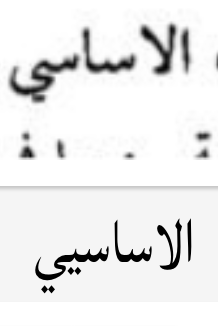
\includegraphics[height=3cm]{images/image20.png}
	\caption{"Doubled Letter" errors}
	\label{fig3:fig4}
\end{wrapfigure}

The “doubled letter” error type was the most frequent that we observed in the
OCR output data (see example in figure~\ref{fig3:fig4}).\footnote{In the images
in figures~\ref{fig3:fig4} to \ref{fig3:fig31}  below the Arabic text at the top
of the images is the original scan and the text below is the OCR output}
                   
At first this error was perplexing. However, it was subsequently discovered
that these “doubling” errors were an artifact of the decoding algorithm
converting the sequence of confidences for each character produced by the
neural network into a series of characters. As the network assigns each
character a probability for each pixel-wide vertical slice of the input line
image and printed characters are wider than a single pixel an algorithm is
needed to extract the actual line text from the longer character probability
sequence. Our implementation was based on a thresholding and merging approach
which can cause doubled characters when the network assigns a probability below
the threshold for a character at a vertical slice between high probability
slices for the same character.\footnote{As a simplified example, assume the
network assigns a probability for character x at 4 vertical slices: $(0.9, 0.95,
0.6, 0.9)$. Decoding with a threshold of $0.5$ will result in an intermediate
sequence xxxx that is then merged to x, while selecting a higher threshold of
$0.7$ will result in a potentially erroneous character sequence of xx merged from
xx\_x.} This error has been effectively addressed by switching to a greedy
decoding which always uses the highest probability character at each vertical
slice.

\subsection{Header/Font Alteration, Footnotes, and Superscript Numerals}

\begin{figure}[h!tp]
	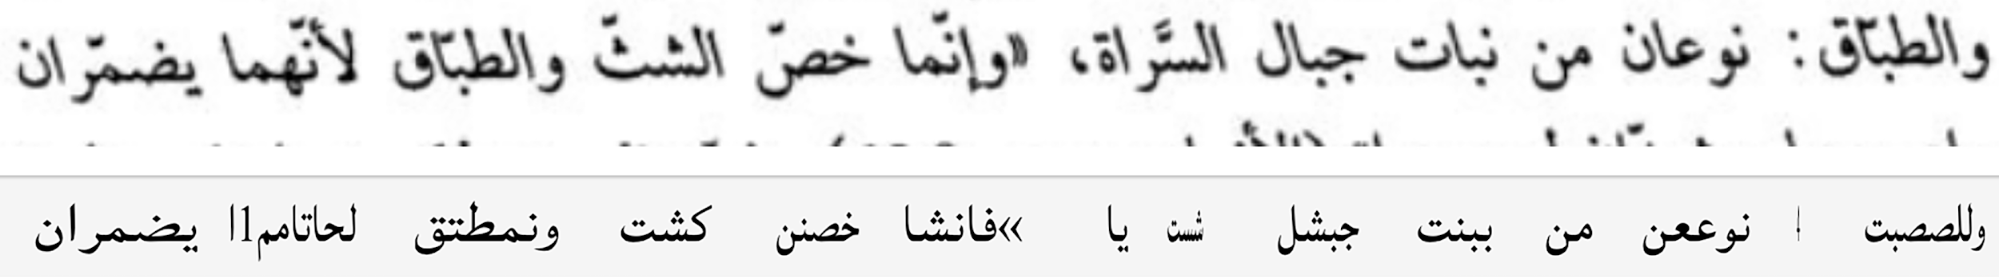
\includegraphics[width=\linewidth]{images/image6.png}
	\caption{Example of poor transcription of italicized passage in figure~\protect\ref{fig3:fig5}}
	\label{fig3:fig6}
\end{figure}


Errors that occured in the context of changes in the font (bolded, italicized,
enlarged/decreased text size) represent the largest category of errors in the
OCR output. Their total numbers are not even fully reflected in Table 3 because
examples in which whole sections (see examples in figures~\ref{fig3:fig5},\ref{fig3:fig6}) were severely
mistranscribed were not enumerated (character-by-character) in the error totals
of the OpenITI manual assessment. Such sections were very rare, and in most
other cases the OCR still rendered text with font alterations with a relatively
high degree of accuracy, but font alterations do seem to increase error rates.

\begin{figure}[h!tp]
	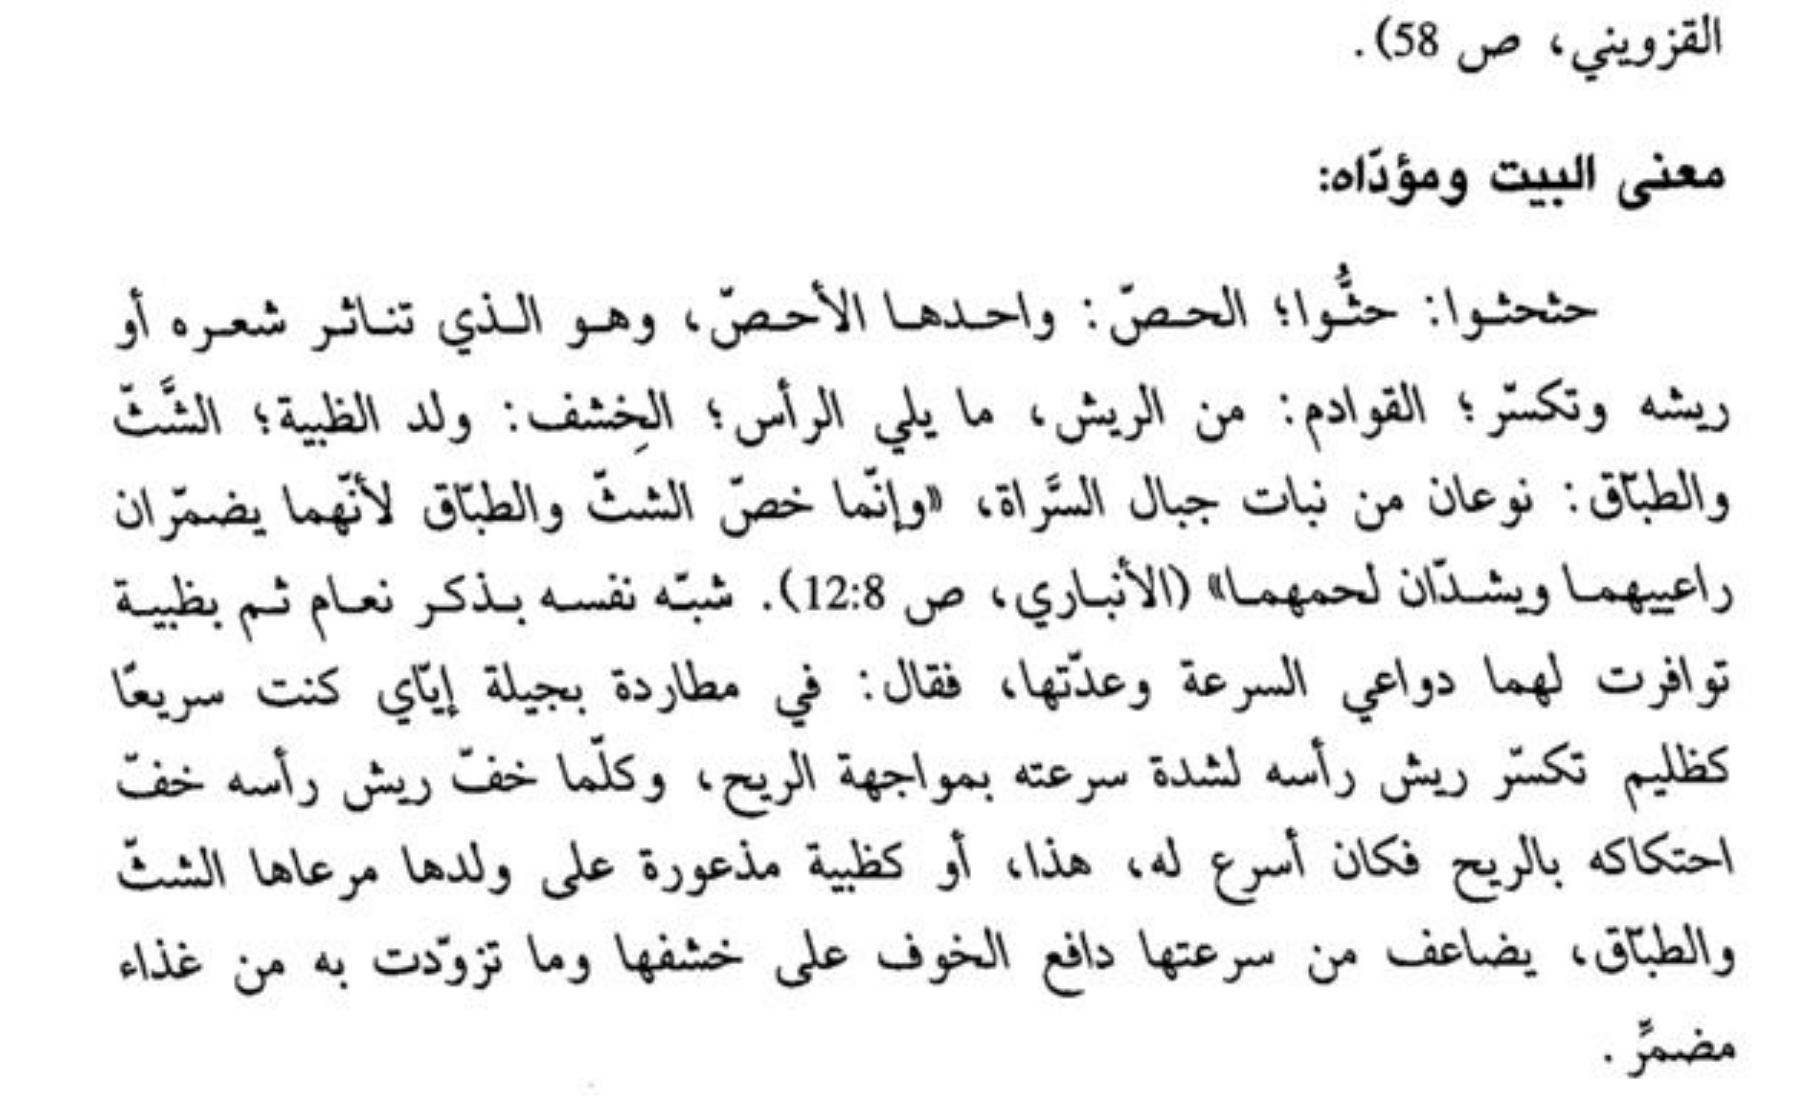
\includegraphics[width=\linewidth]{images/image19.png}
	\caption{Example of text in italics}
	\label{fig3:fig5}
\end{figure}

One of the most common examples of this issue was observed in text headers
(including both section headers and chapter titles), which were typically
bolded or bolded and enlarged in al-Abhath (see figure~\ref{fig3:fig7}). In some
headers, as mentioned above, an entirely different typeface was employed (see
figure~\ref{fig3:fig3}) -- although this is a less common practice.

\begin{figure}[h!tp]
	\centering
	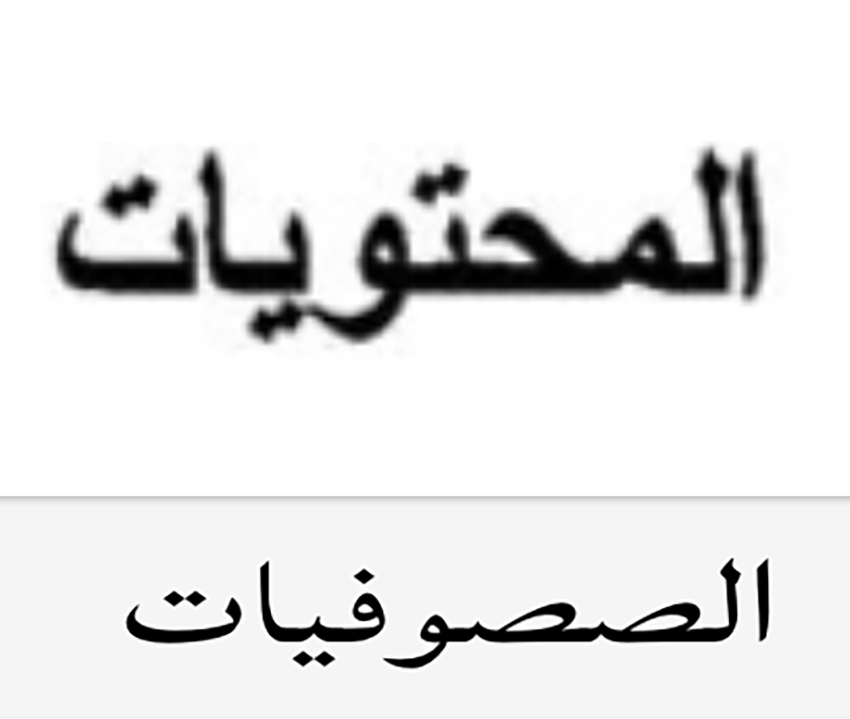
\includegraphics[height=3cm]{images/image5.png}
	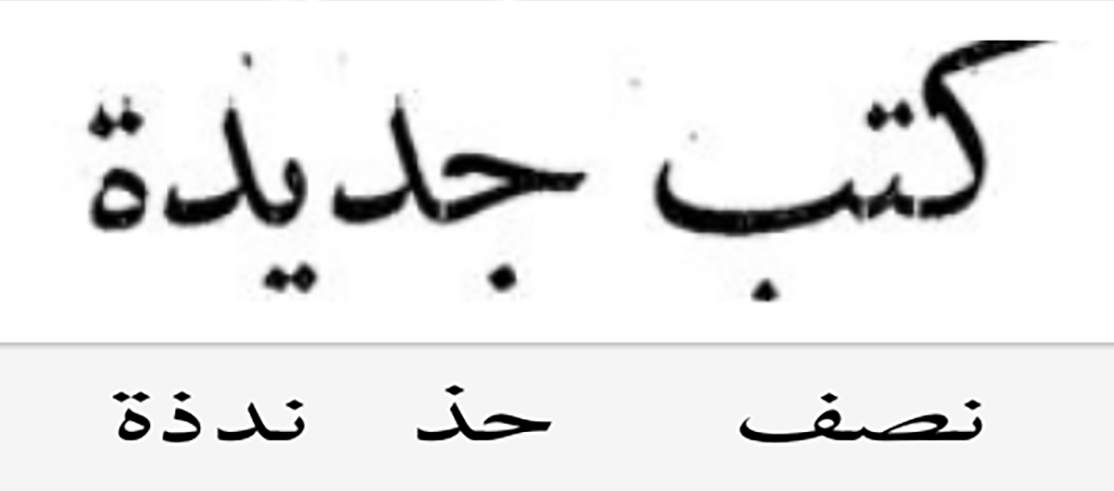
\includegraphics[height=3cm]{images/image7.png}
	\caption{Bolded and enlarged text size header and poor transcription}
	\label{fig3:fig7}
\end{figure}

Other modifications to the font of the typeface, e.g., footnotes, superscript
(decreased text size) numerals, also seem to be correlated with decreased
accuracy rates. In the future, this could be addressed by ensuring that a
sufficient number of lines of training data with such font modifications is
included.

\subsection{Ligatures/Atypical Letter or Dot Forms}

Not surprisingly, ligatures and other types of less common letter patterns and
dot placements led to less accurate transcriptions in the OCR output (see
figure~\ref{fig3:fig914}). This same problem has been observed in an earlier study as well \cite{kiessling2017important}.

\begin{figure}[!ht]
	\centering
	\begin{subfigure}[t]{0.3\linewidth}
	\centering
	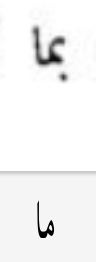
\includegraphics[height=3cm]{images/image21.png}
	\caption{Example of problematic ligature and error in transcription}
	\label{fig3:fig9}
	\end{subfigure}
	\begin{subfigure}[t]{0.3\linewidth}
	\centering
	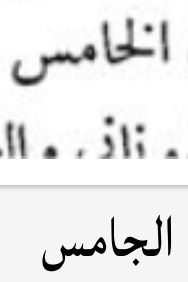
\includegraphics[height=3cm]{images/image23.png}
	\caption{Example of problematic ligature and error in transcription}
	\label{fig3:fig10}
	\end{subfigure}
	\begin{subfigure}[t]{0.3\linewidth}
	\centering
	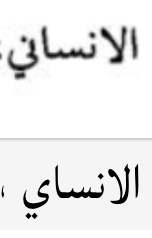
\includegraphics[height=3cm]{images/image22.png}
	\caption{Atypical dot placement}
	\label{fig3:fig11}
	\end{subfigure}

	\begin{subfigure}[t]{0.3\linewidth}
	\centering
		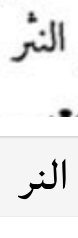
\includegraphics[height=3cm]{images/image26.png}
	\caption{Atypical dot placement}
	\label{fig3:fig12}
	\end{subfigure}
	\begin{subfigure}[t]{0.3\linewidth}
	\centering
	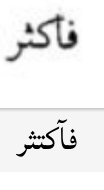
\includegraphics[height=3cm]{images/image24.png}
	\caption{Atypical letter pattern (printing error?)}
	\label{fig3:fig13}
	\end{subfigure}
	\begin{subfigure}[t]{0.3\linewidth}
	\centering
	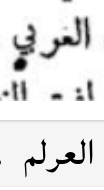
\includegraphics[height=3cm]{images/image25.png}
	\caption{Atypical dot/letter placement and poor scan quality}
	\label{fig3:fig14}
	\end{subfigure}
	\caption{Ligatures and uncommon letter patterns}
	\label{fig3:fig914}
\end{figure}

It is nearly impossible to completely avoid this problem, but a more systematic
approach to training data generation that selected pages/lines of data with an
eye towards ensuring sufficient representation of the maximum number of
ligatures could improve OCR accuracy on these characters/character
combinations.

\subsection{Diacritics}

\begin{figure}[!ht]
	\centering
	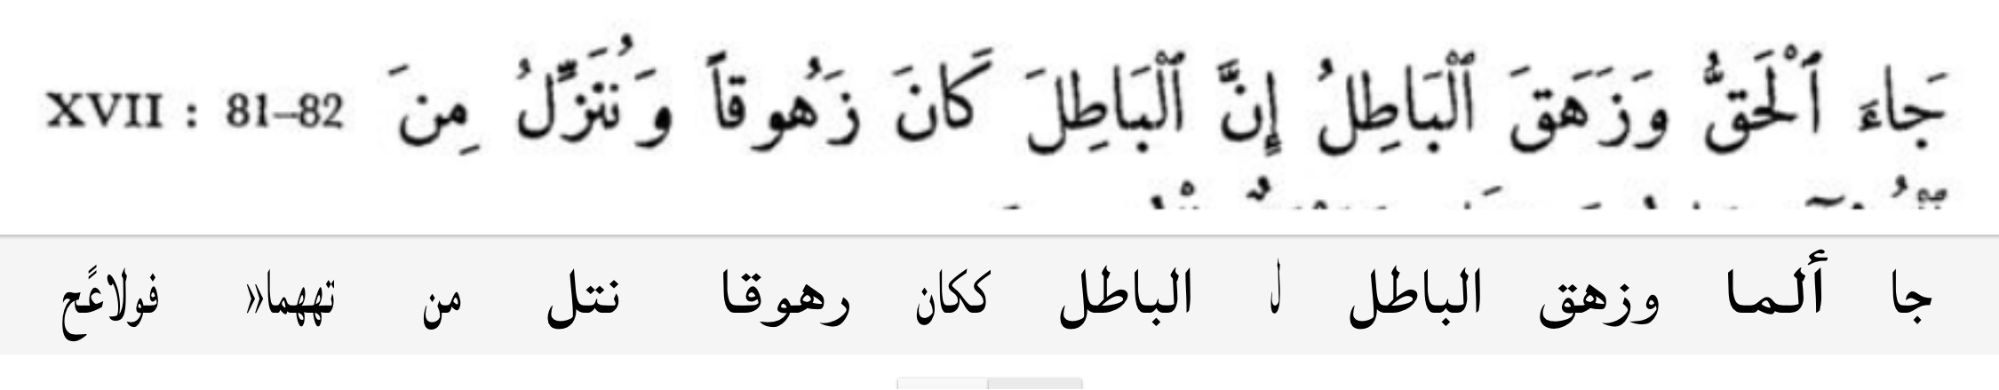
\includegraphics[width=\textwidth]{images/image27.png}
	\caption{Highly vocalized Qur’anic passage that is transcribed poorly due to diacritics}
  	\label{fig3:fig15}
\end{figure}

Words that contained diacritics also appear more frequently to have errors in
transcription, which leads us to believe that diacritics are interfering with
character recognition. This tendency especially can be seen in examples of
heavy vocalization, such as the fully vocalized Qur’anic passage seen in
figure~\ref{fig3:fig15}, which are poorly transcribed. Figure~\ref{fig3:fig15}
is an extreme case that is an outlier in the al-Abhath data, but it clearly
illustrates this problem.  Moreover, although al-Abhath journal articles are
not heavily vocalized, this could be a significant issue in other Arabic texts
that are heavily vocalized. 

\begin{figure}
	\centering
	\begin{subfigure}[t]{0.45\linewidth}
		\centering
	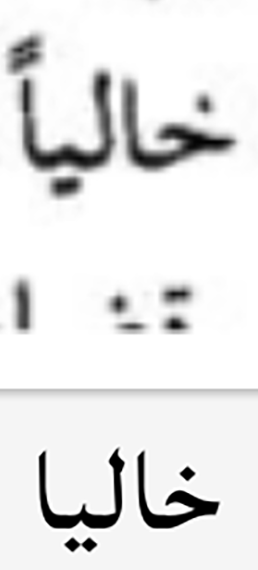
\includegraphics[height=3cm]{images/image3.png}
	\caption{Missed fatḥa tanwīn}
  	\label{fig3:fig16}
	\end{subfigure}
	\begin{subfigure}[t]{0.45\linewidth}
	\centering
	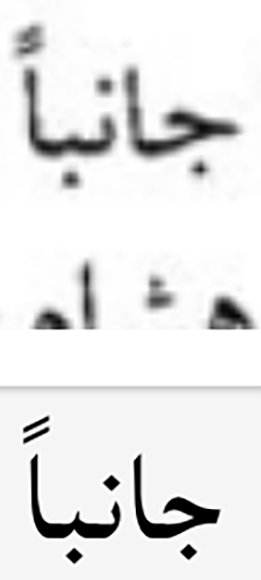
\includegraphics[height=3cm]{images/image1.png}
	\caption{Correctly transcribed fatḥa tanwīn from same page as figure~\protect\ref{fig3:fig16}.}
  	\label{fig3:fig17}
	\end{subfigure}
	\caption{Transcription of fatḥa tanwīn}
\end{figure}

In general, OpenITI has traditionally followed the practice of not transcribing
Arabic diacritics in our training data production (with one exception discussed
below). We have followed this practice for three reasons: (1) vocalization is
often inconsistent and sometimes incorrect (so it is better to allow the
individual scholar to determine the proper vocalization based upon their
reading); (2) vocalization can interfere with computational textual analysis
(computational linguists, for example, typically remove it in their
normalization of texts in preparation for analysis); and, (3) not all full-text
search algorithms support diacritics in a useful way. There is one problem with
this approach, however, that we have found in both this study and another
concurrent one on Persian OCR. If there is a sufficient amount of diacritics in
the original text, the model will “learn” to ignore diacritical marks and it
will not interfere with character recognition. However, if the original text is
lightly vocalized and not enough examples of diacritics are contained in the
training data, then it appears that the model does not “learn” well enough to
ignore the diacritics and thus their presence in a word interferes with
accurate character recognition. This situation presents us with a dilemma
around which we need to develop a set of guidelines: we do not want to include
diacritics because of the aforementioned reasons and because including them in
the training data will require even more time expenditure in the training data
generation process, but by not including them in texts with light vocalization
(e.g., al-abhath, some of the Persian texts in our other tests) character
recognition is reduced in words with them. 

\subsection{Missed Fatḥa Tanwīn}

The exception to our traditional treatment of diacritics discussed in the
previous section is the case of the Arabic diacritic fatḥa tanwīn (\textarabic{اً}). As
observed in the CER reports, missed fatḥa tanwīns were a significant source of
errors. We also observed this in the manual review of the OCR output (see
figure~\ref{fig3:fig16}).

Although in the past we have not transcribed fatḥa tanwīns in the training data
production process, we did include fatḥa tanwīns in the JSTOR pilot training
data. In many cases the fatḥa tanwīns were transcribed correctly (see
figure~\ref{fig3:fig17} for comparison sake). However, as both the CER reports
and manual review showed, they still remained a relatively common source of
errors.  The reason(s) that fatḥa tanwīn remained a problem in the
transcription process could be related to either (1) its lack of sufficient
representation in the training data, or (2) its position in the line
segment—i.e., in some cases it might be partially getting cut off since it
appears so high in the line segment box. In either case, we are inclined to
ignore fatḥa tanwīns in future training data production. 

\subsection{Punctuation Marks, Number, and Other Non-Alphanumeric Symbols}

Punctuation marks, numbers, and other non-alphanumeric symbols (e.g.,
\$) - especially representatives of each of these categories that were less
commonly used in al-Abhath - were another recurring source of errors. The way to
address this problem is by making sure these signs, symbols, and numbers are
sufficiently represented in the training data.

\subsection{Hamzas}

\begin{figure}[H]
	\centering
	\begin{subfigure}[t]{0.3\linewidth}
	\centering
	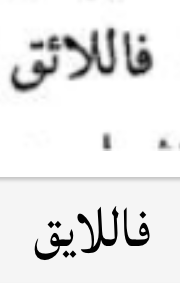
\includegraphics[height=3cm]{images/image28.png}
	\caption{Missed hamza}
	\label{fig3:fig18}
	\end{subfigure}
	\begin{subfigure}[t]{0.3\linewidth}
	\centering
	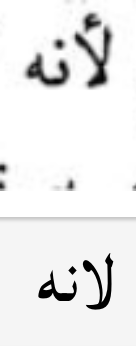
\includegraphics[height=3cm]{images/image29.png}
	\caption{Missed hamza on alif}
	\label{fig3:fig19}
	\end{subfigure}
	\begin{subfigure}[t]{0.3\linewidth}
	\centering
	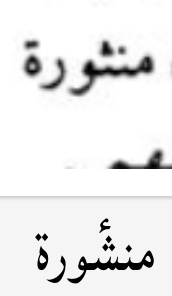
\includegraphics[height=3cm]{images/image30.png}
	\caption{Inserted extra hamza}
	\label{fig3:fig20}
	\end{subfigure}
	\caption{Misrecognized hamzas}
	\label{fig3:fig1820}
\end{figure}

The hamza character was another common source of errors in the output, both in
the sense that it was misrecognized (see figure~\ref{fig3:fig1820}) and inserted
in instances in which it was not in the original scan (see
figure~\ref{fig3:fig20}). 

Again, this is a case in which more focused training data will improve
recognition rates—an intervention we must make at the training data generation
phase of the OCR process.  

\subsection{Atypical Text Presentation Format and Kashīda/tatwīl (elongation character)}

There are a series of errors that occur in the context of atypical presentation
formats/atypical character patterns. These range from the use of the Arabic
elongation character (kashīda/tatwīl) (see figure~\ref{fig3:fig21}) to various types of table
formats (see figures~\ref{fig3:fig22},\ref{fig3:fig23},\ref{fig3:fig24}).

\begin{figure}
	\centering
	\begin{subfigure}[t]{0.48\linewidth}
	\centering
	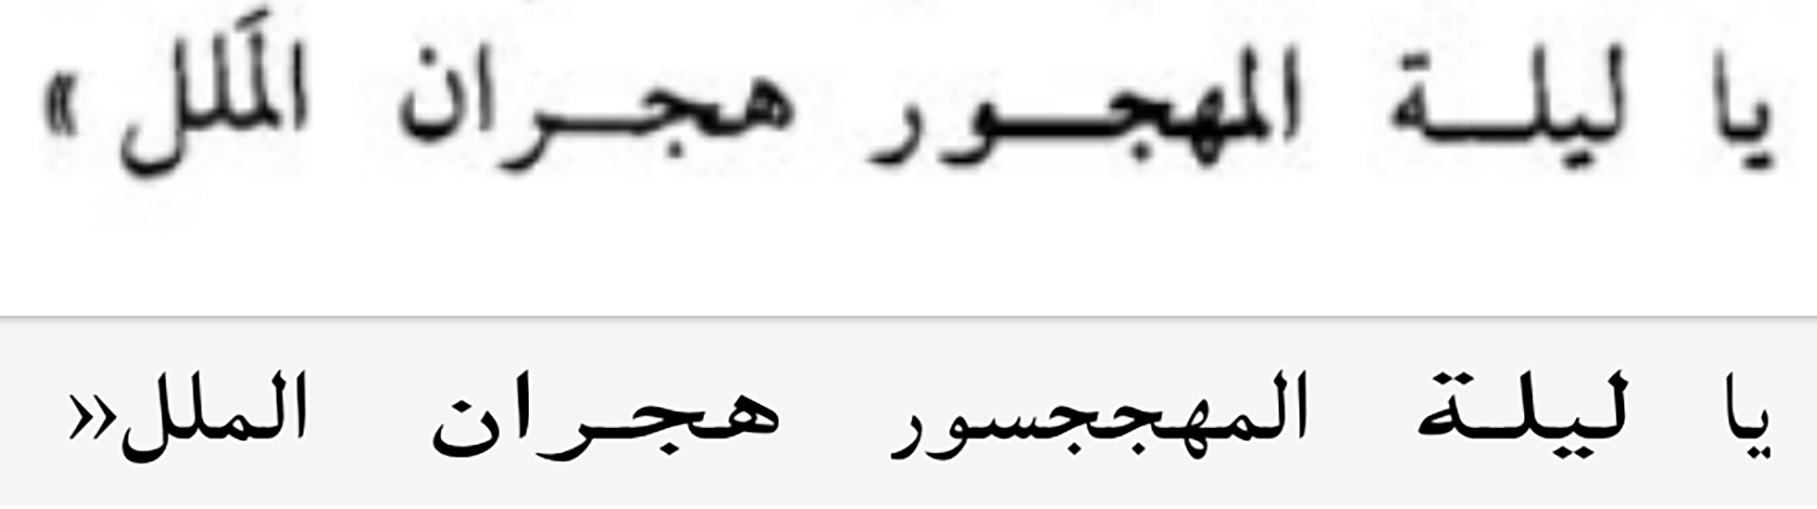
\includegraphics[width=\textwidth]{images/image2.png}
	\caption{Read letter ‘sin’ into word due to kashīda/tatwīl (elongation).}
	\label{fig3:fig21}
	\end{subfigure}
	\begin{subfigure}[t]{0.48\linewidth}
	\centering
	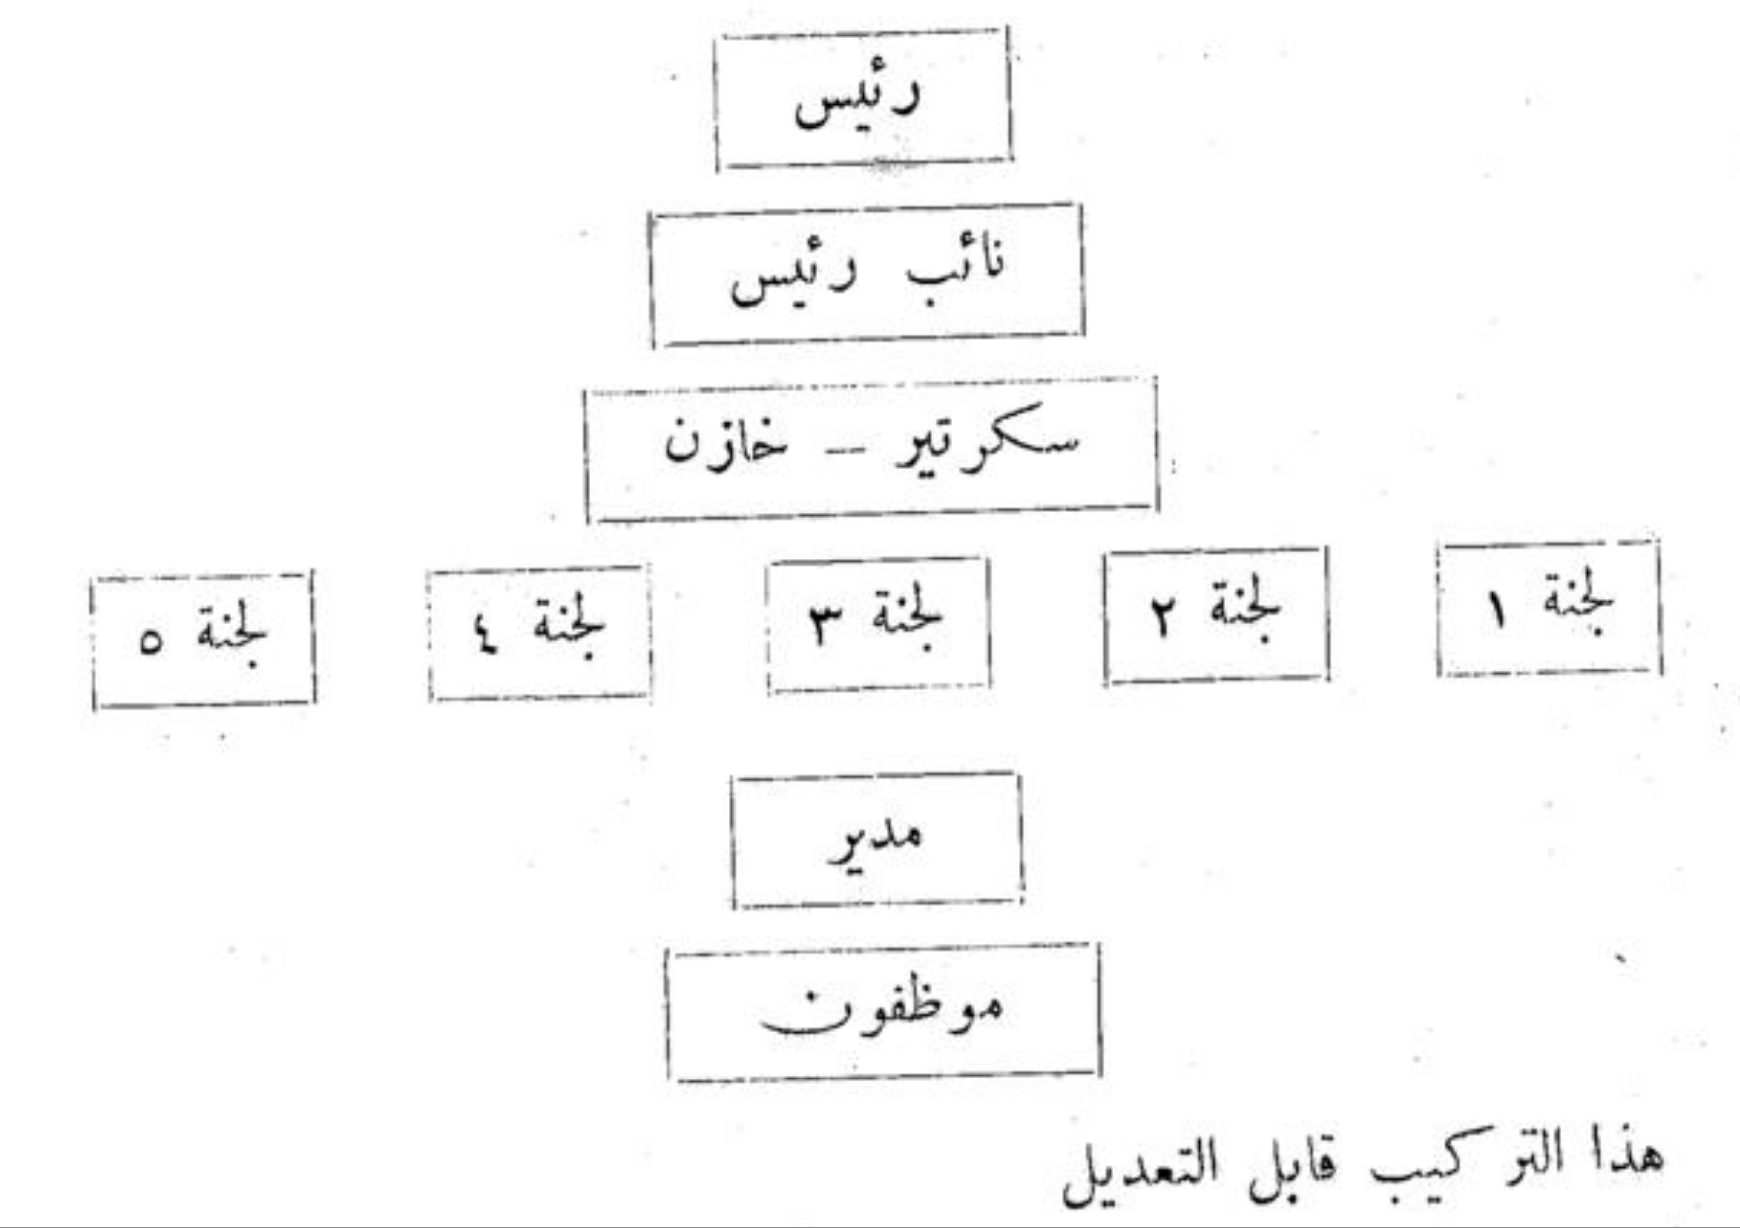
\includegraphics[width=\textwidth]{images/image31.png}
	\caption{Example of table format}
	\label{fig3:fig22}
	\end{subfigure}
	\vskip\baselineskip
	\begin{subfigure}[t]{0.48\linewidth}
	\centering
	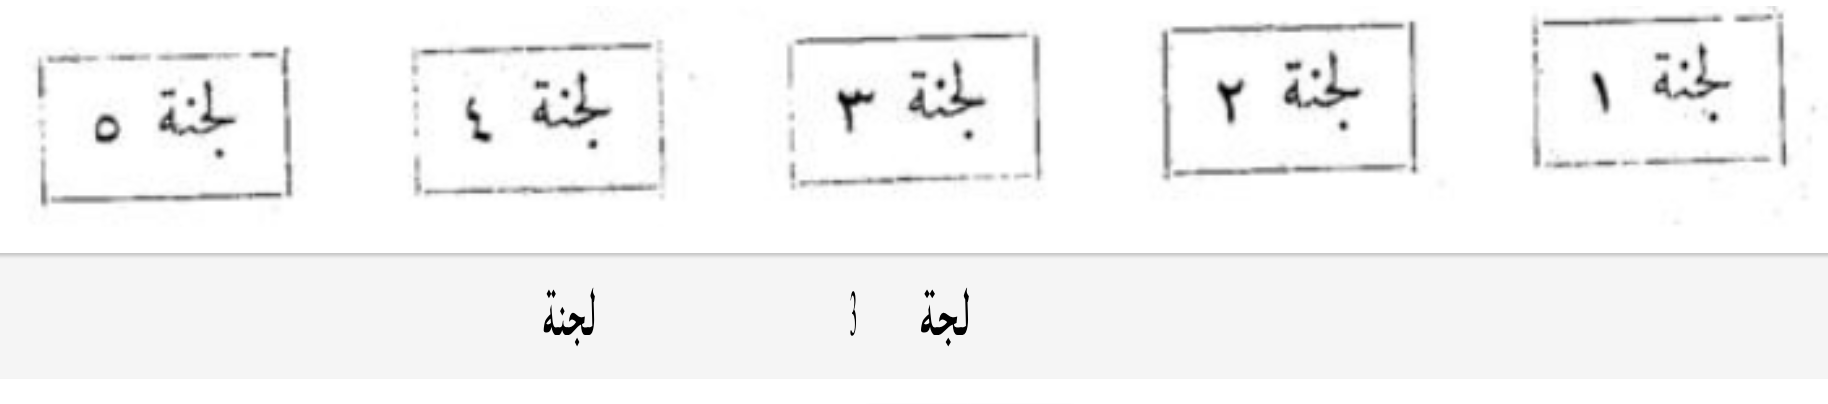
\includegraphics[width=\textwidth]{images/image10.png}
	\caption{Example of particularly poor transcription on an atypical (table) presentation format.}
	\label{fig3:fig23}
	\end{subfigure}
	\begin{subfigure}[t]{0.48\linewidth}
	\centering
	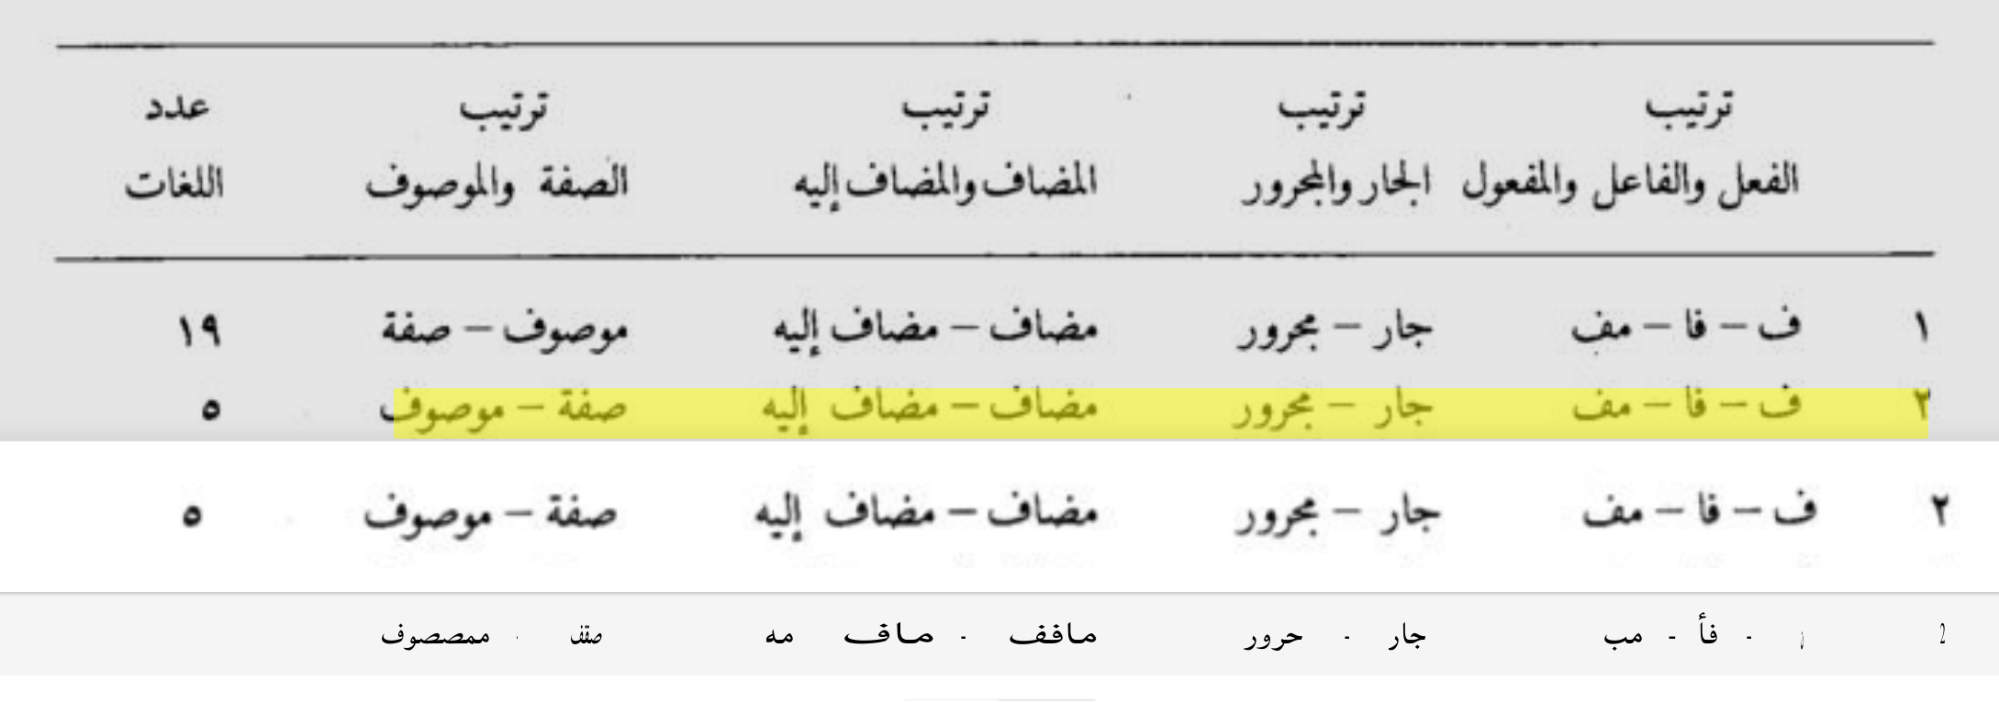
\includegraphics[width=\textwidth]{images/image11.png}
	\caption{Example of particularly poor transcription on another atypical
(table) presentation format\footnote{Full view of our OCR post-correction
interface is shown in figures~\ref{fig3:fig2124},~\ref{fig3:fig25} in order to
show the broader page context from which the highlighted lines are drawn and
displayed in a line pair (image of line and its digital transcription) in the
pop-up. Specifically, please note that in figure~\ref{fig3:fig24} this line is
drawn from a larger table and in figures~\ref{fig3:fig25},~\ref{fig3:fig26} this line is
drawn from a page with significant admixture of both Arabic and Persian in the
text.}.}
	\label{fig3:fig24}
	\end{subfigure}
	\caption{Atypical presentation forms}
	\label{fig3:fig2124}
\end{figure}

Although the character recognition in these examples is usually not as poor as
in figure~\ref{fig3:fig23}, we still observed that errors seem to appear more
frequently in such contexts (see the better recognition in
figures~\ref{fig3:fig21} and ~\ref{fig3:fig24}). More training data from these
atypical presentation formats and character patterns will help improve
accuracy, but improvements in line segmentation are also necessary for such
examples as figure~\ref{fig3:fig23}.

\subsection{Non-Arabic Language}

\begin{figure}[H]
	\centering
	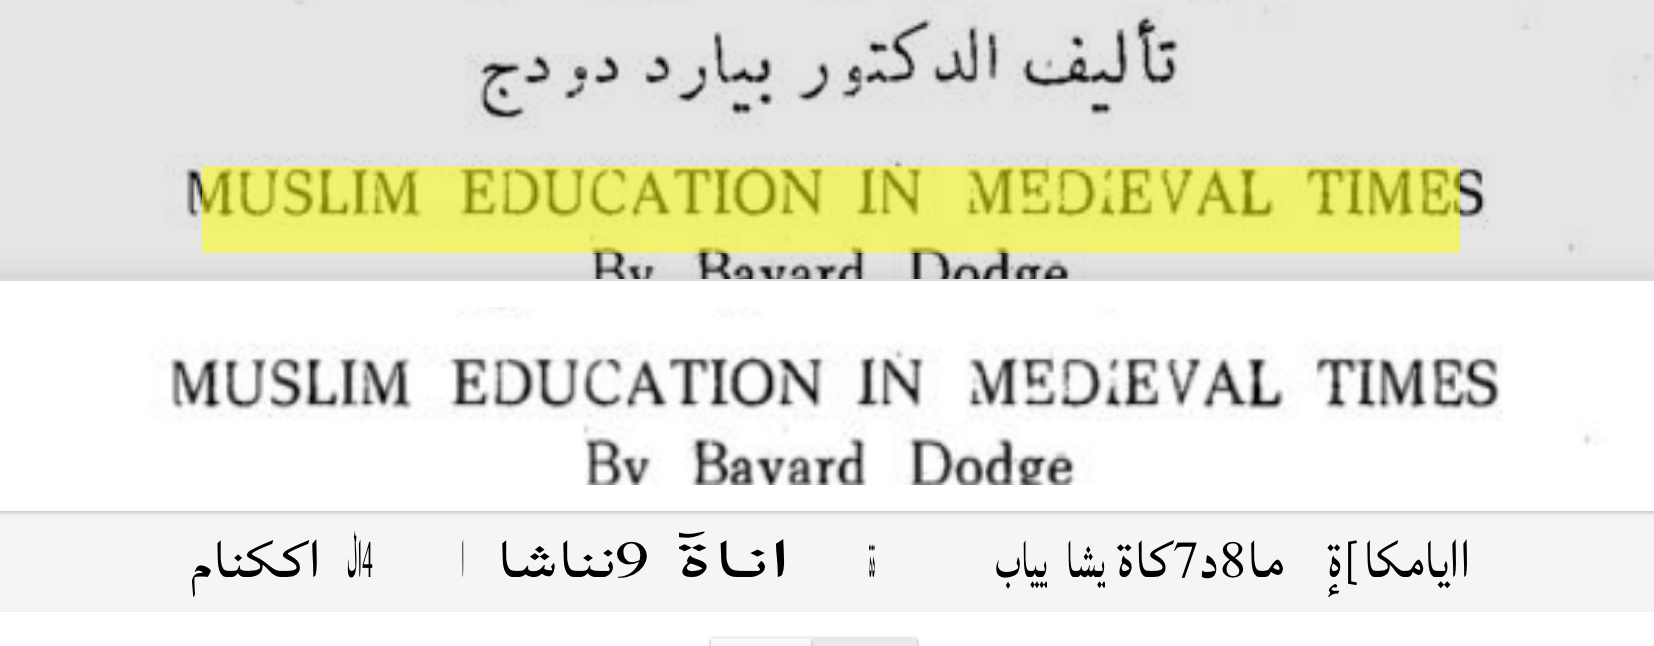
\includegraphics[width=0.7\linewidth]{images/image12.png}
	\caption{Example of particularly poor transcription of non-Arabic language in a page of primarily Arabic text.}
	\label{fig3:fig25}
\end{figure}

There were two significant types of transcription errors that were related to
the presence of non-Arabic language in the original text. The first, seen in
figure~\ref{fig3:fig25}, is the poor transcription of non-Arabic characters on a
page that predominantly contains Arabic text. (Figure~\ref{fig3:fig25}
represents a particularly poor transcription of the non-Arabic text; most
transcriptions in such instances were much more accurate.)
  
The second type of error that occurred in the context of non-Arabic script was
the inverse: that is, poor transcription of Arabic text on a page that is
predominantly composed of a non-Arabic language (see figure~\ref{fig3:fig26}). 

\begin{figure}[H]
	\centering
	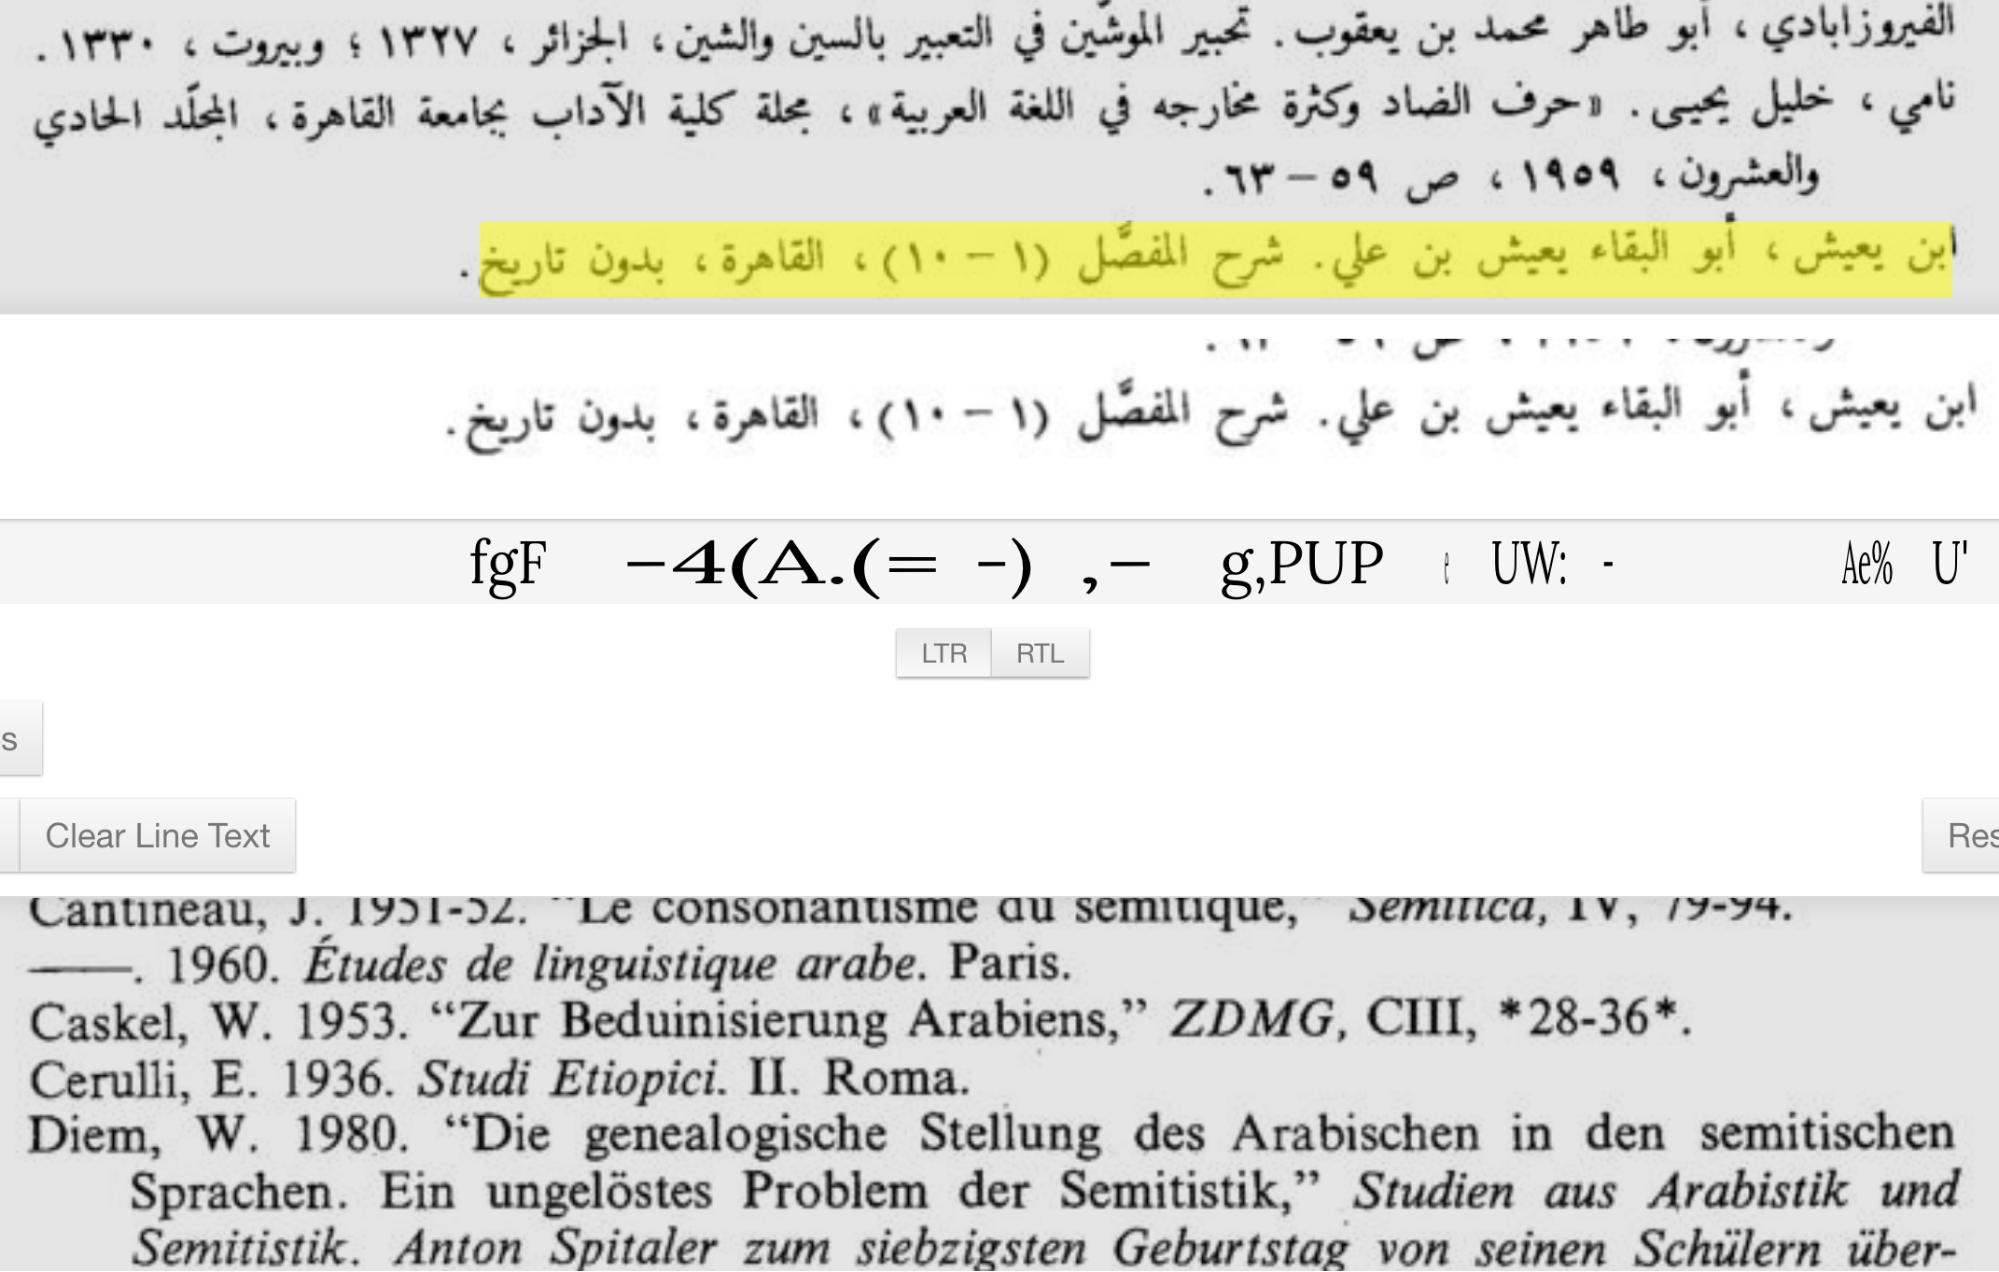
\includegraphics[width=0.7\linewidth]{images/image13.png}
	\caption{Page with substantial non-Arabic language interferes with Arabic OCR.}
	\label{fig3:fig26}
\end{figure}
 
This is a known problem that can be addressed through the development of
multi-language OCR models - a project that OpenITI is currently working on.

\subsection{Poor Scan Quality}

\begin{figure}[H]
	\centering
	\begin{subfigure}[t]{4cm}
	\centering
	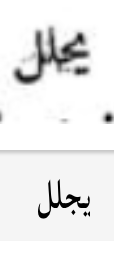
\includegraphics[height=4cm]{images/image14.png}
	\caption{Black shading in background of letters.}
	\label{fig3:fig27}
	\end{subfigure}
	\begin{subfigure}[t]{4cm}
	\centering
	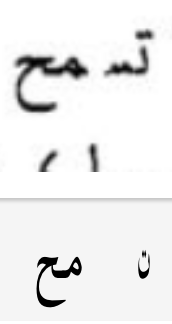
\includegraphics[height=4cm]{images/image15.png}
	\caption{Missing print in letter.}
	\label{fig3:fig28}
	\end{subfigure}
	\caption{Examples of poor scan quality}
\end{figure} 

Poor scan/print quality—including, errant marks (see figure~\ref{fig3:fig27}), lack of ink
(see figure~\ref{fig3:fig28}), misplaced letters/punctuation (figure~\ref{fig3:fig13}) - is not a
particularly common source of errors in the al-Abhath data, but there is a
critical mass of errors caused by this problem.

This problem cannot be addressed in the OCR process. OCR accuracy is
(obviously) limited by the quality of the original scans.

\subsection{Line Segmentation}

\begin{figure}[H]
	\centering
	\begin{subfigure}[b]{0.48\linewidth}
	\centering
	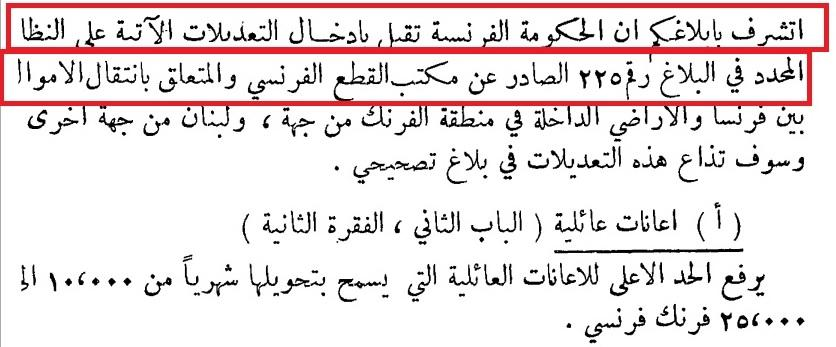
\includegraphics[width=\linewidth]{images/image16.jpg}
	\caption{Missed line segments (from outside contractor accuracy review).}
	\label{fig3:fig29}
	\end{subfigure}
	\begin{subfigure}[b]{0.48\linewidth}
	\centering
	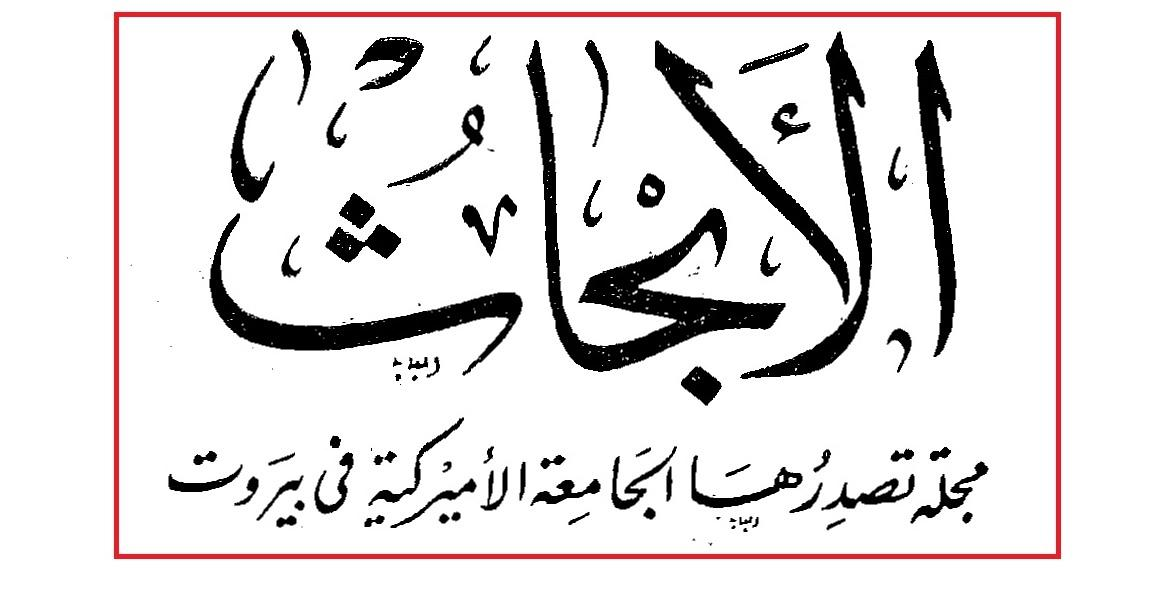
\includegraphics[width=\textwidth]{images/image17.jpg}
	\caption{Large header segmented as one line (from outside contractor accuracy review).}
	\label{fig3:fig30}
	\end{subfigure}
	\caption{Examples of missegmentation}
	\label{fig3:fig2930}
\end{figure} 

One final error type that should be mentioned is line segmentation errors (see
figures~\ref{fig3:fig2930},\ref{fig3:fig31}). 

This type of error was not commonly found in the OpenITI manual accuracy
assessment (figure~\ref{fig3:fig2930} were errors identified in the outside contractor’s
review of the OCR output), but there were a few cases in which the line
segmenter missed a section or a word of a line. Typically this would occur in
atypical text presentation formats, such as the table seen in figure~\ref{fig3:fig31}.

\begin{figure}[h]
	\centering
	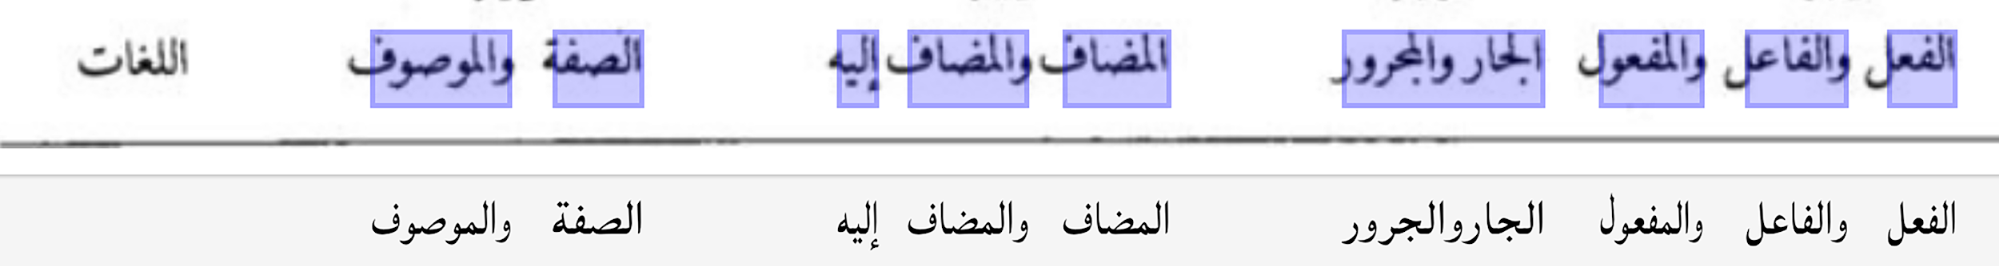
\includegraphics[width=\linewidth]{images/image4.png}
	\caption{Line segmenter missed final word in the line.}
	\label{fig3:fig31}
\end{figure} 

Truncation of Arabic text lines is a known problem for the
Latin-script-op\-tim\-iz-ed line segmenter in the version of Kraken that was used
for this study. The implementation of a novel trainable layout analysis method
has largely solved this issue\cite{kiessling2019badam}.

\sectionmark{Recommendations for Arabic-script OCR}
\section{Recommendations and Future Avenues of Development for Open Source Arabic-script OCR}

The results of this study indicate that work in the following three areas could
generate significant improvements for open source Arabic-script OCR: 

\begin{enumerate}
\item Systematic training data production. Instead of generating training data
in a completely randomized (or haphazard) manner (as is often
done),\footnote{We followed this randomized training data generation approach
in the past \cite{kiessling2017important}. See \cite{springmann2018ground} for
an example of a dataset resulting from haphazard convenience sampling, i.e.
harvesting data from sources on which existing methods already produce
near-perfect results.} future Arabic-script OCR projects need to study the
particularities of the documents they plan to OCR and make sure that the pages
selected for training data production contain a sufficient number of the less
common ligatures, headers, diacritics, footnote text, numbers, and other
particularities of the works to be OCR’d. This more systematic approach to
training data production will require more time upfront. But the models
produced in this manner could potentially achieve much higher baseline accuracy
and reduce the burden of postcorrection. 
\item Generalized models. One of the most exciting results from this study was
the significant improvements in accuracy achieved with the generalized Arabic
model. The success of this approach tentatively suggests that if we continue to
add training data sets to this generalized model we can anticipate to achieve
higher levels of accuracy on both typefaces on which we have already trained
models and new typefaces for which we have no training data yet. If this
pattern holds true in future studies, we would be able to gradually reduce the
time and resources necessary to achieve high level accuracy (>97\%) on new
typefaces in the future. However, more research on generalized models is needed
as both the optimal training data selection, including artificial data produced
by methods such as \cite{milo2019new}, for such models and the actual
variance on an open text corpus is currently unknown.
\item There are a range of technical improvements—e.g., multi-language models,
improved line segmentation and layout analysis—that could significantly improve
OCR accuracy numbers. Efforts are currently underway in both the eScripta
project (of which Kiessling is a team member) and OpenITI’s Arabic-script OCR
Catalyst Project (AOCP) to address each of these technical issues.\footnote{For
more information on the eScripta project, please see:
\url{https://escripta.hypotheses.org/}. For more information on OpenITI’s AOCP
project, please see: \url{https://openiti.org/projects/openitiaocp}.}
\end{enumerate}

\section*{Acknowledgements}

We would also like to thank David Smith (Northeastern University) for his
suggestions and feedback on this study. This work was supported by a subgrant
from JSTOR from their National Endowment for the Humanities-funded feasibility
study on high-quality digitization and digital preservation of Arabic scholarly
journals (grant number PW-253861-17).


\section*{Competing Interests}

This work was supported by a subgrant from JSTOR from their National Endowment
for the Humanities-funded feasibility study on high-quality digitization and
digital preservation of Arabic scholarly journals (grant number PW-253861-17).

\section*{Author Roles}

Authors are listed in alphabetical order. The corresponding author is mtm.
\begin{description}
\item[Conceptualization] bk, mtm
\item[Data curation] bk, gk, mtm, ks
\item[Formal analysis] bk
\item[Funding acquisition] mtm
\item[Investigation] bk, gk, mtm, ks
\item[Methodology] bk, mtm
\item[Project administration] mtm
\item[Resources] bk, mtm
\item[Software] bk
\item[Supervision] mtm
\item[Validation] bk
\item[Visualization] bk, mtm
\item[Writing - original draft] bk, mtm
\item[Writing - review \& editing] bk, gk, mtm, ks
\end{description}
